\section{Additional comments}
Here it follows a list of consideration and comments, that we would like to point out:
\begin{itemize}
\item The implementation and testing document, in our opinion, misses some points. 
In particular, a discussion on how the frameworks adopted match, in some sense, the requirements and the goal of the project 
is not present at all: what is possible to find is only a list of advantages and disadvantages of the framework, and most of them are not
related to the system developed, but very general
\item Motivations regarding the choice of implemented features of automated SOS is not present at all
\item In the section regarding the test, it is said that "tests were done by hand"
This choice has not been motivated and, of course, it presents obvious disadvantages: it is necessary to repeat all the tests as soon as
an update or fix is released
\item Most of the code that we looked at, in particular the backend, misses most of the documentation. For very few methods, some sort
of comments is present
\item It is not clear why, for accepting a request, it is requested to use also the SSN: the token should be the only thing relevant, from a
API design point of view
\item No information regarding the coverage of the test is present in the documentation provided; in our opinion, this is an important information for the stakeholders.

\item While searching for individual data, if a wrong SSN is inserted first, and then 
a correct one, the error message does not disappear. 

\begin{figure}[H]
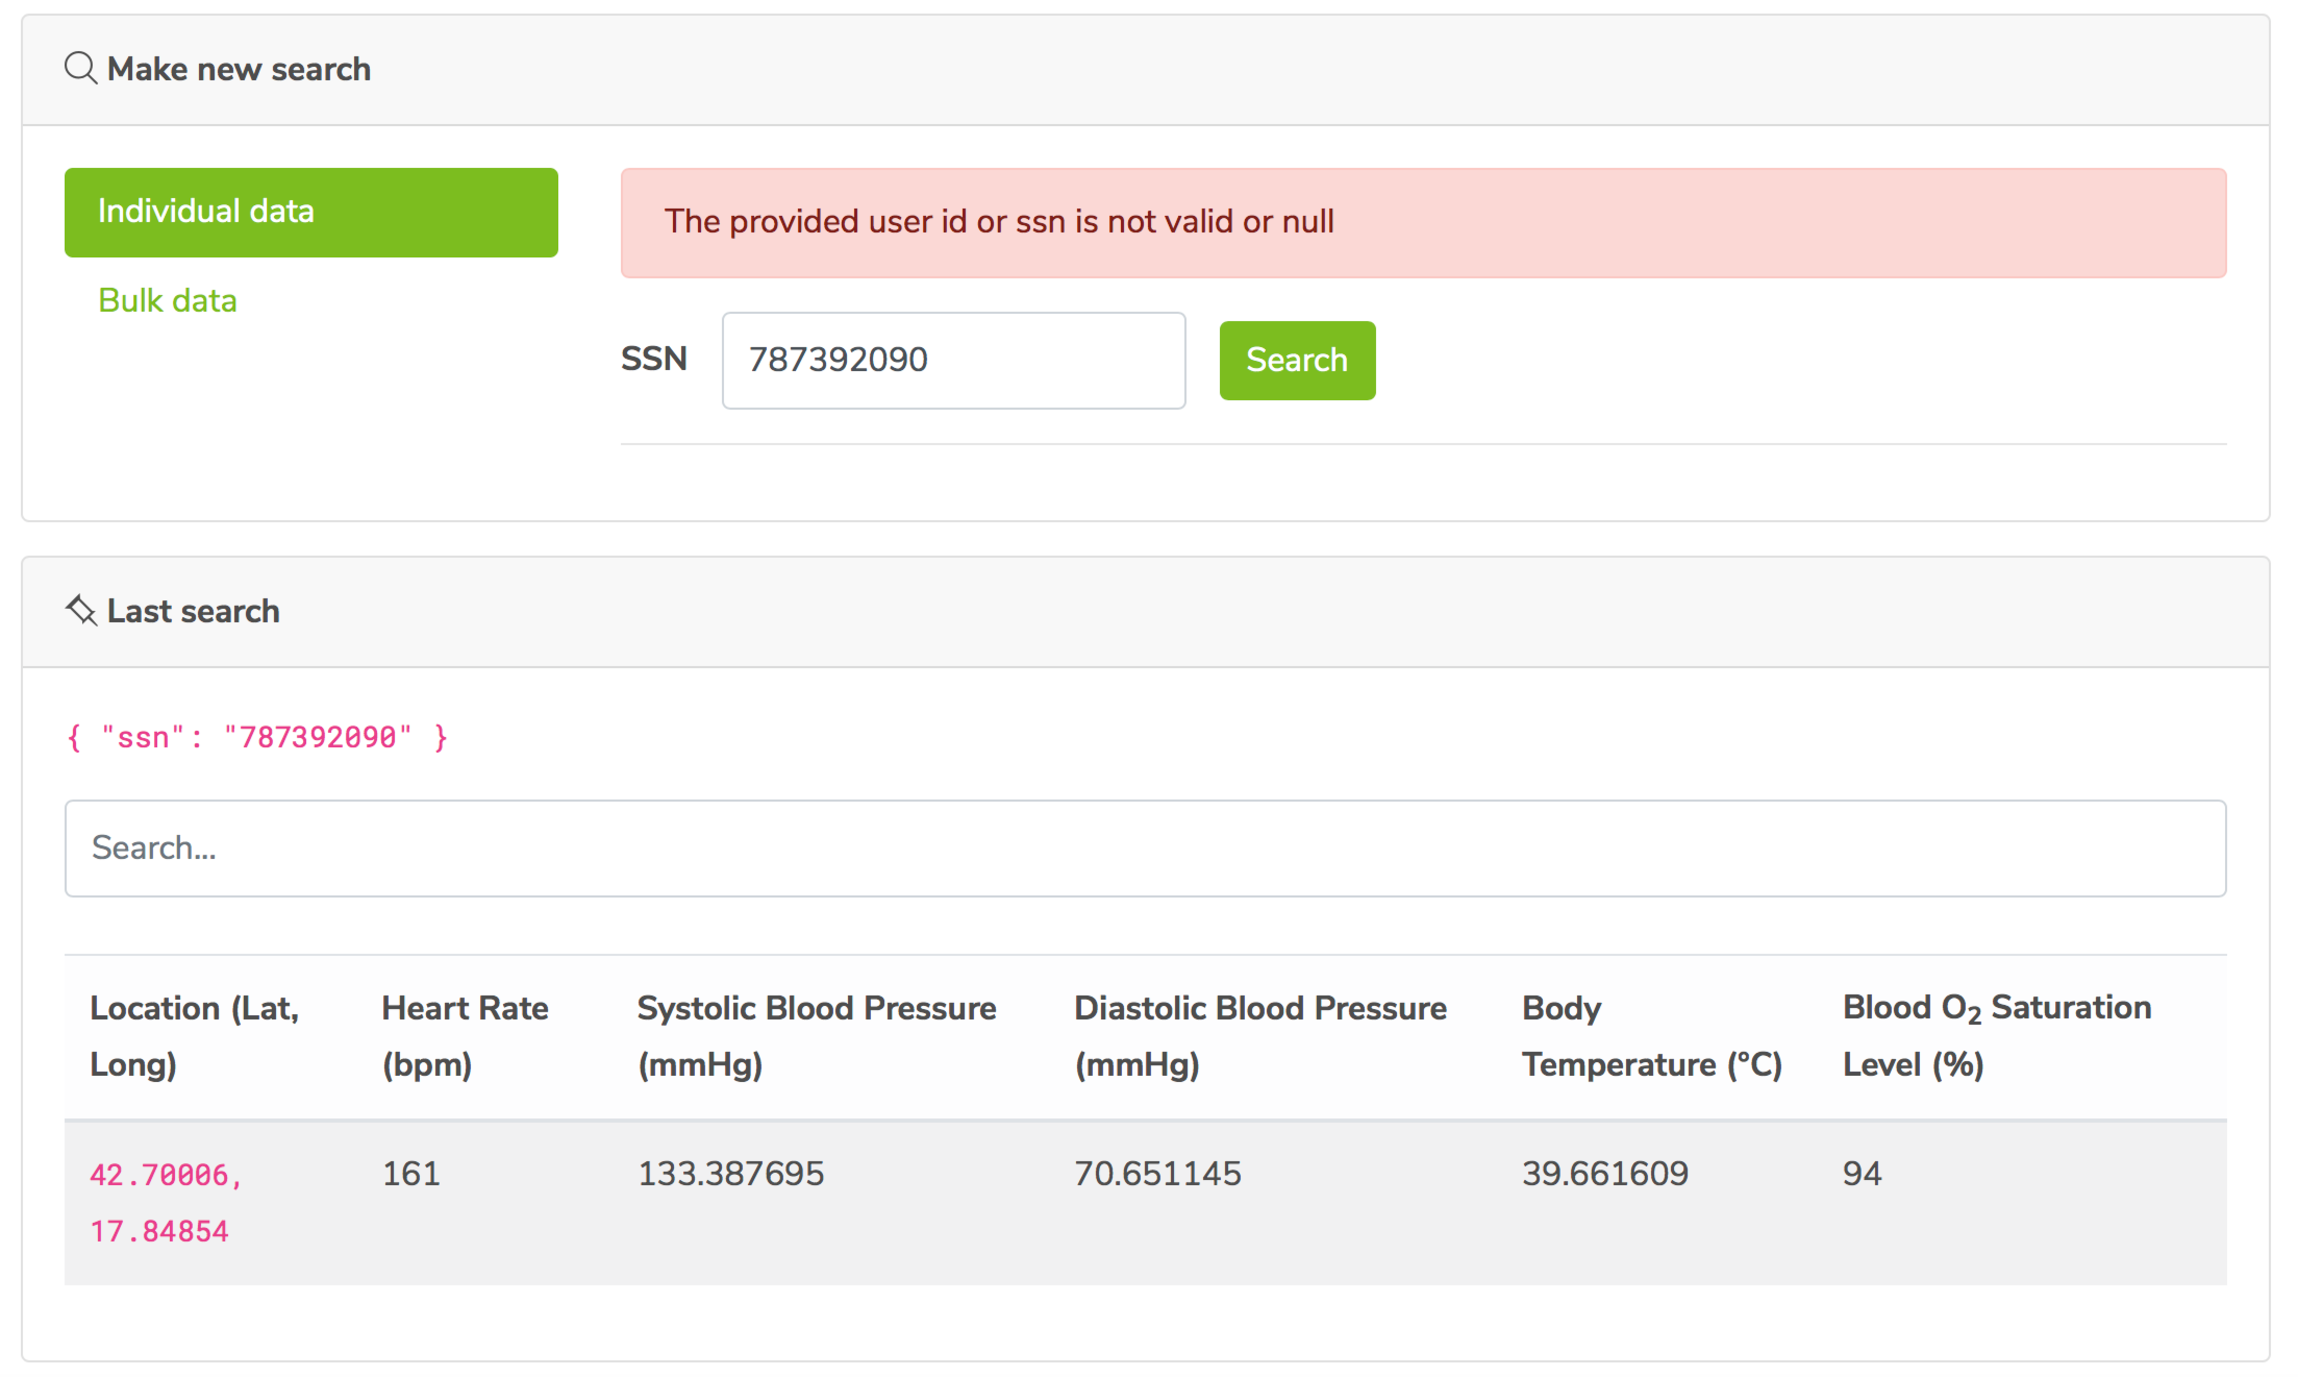
\includegraphics[width=\linewidth]{images/individualCorrectSsn2}
\caption{ UI bug }
\label{fig:bug1}
\end{figure}

Other mini bugs like this are present. However, they are not important since the 
UI is not considered to be the main purpose of the project. \\
This one has been reported as an example, for the sake of completeness.

\item 
On Safari there are some problem with the registration: first it is impossible load a
certificate during the third party registration, in fact though the user manages to load the
certificate, the system always returns an error message saying it is missing. Secondly, the
date picker is not working.

\begin{figure}[H]
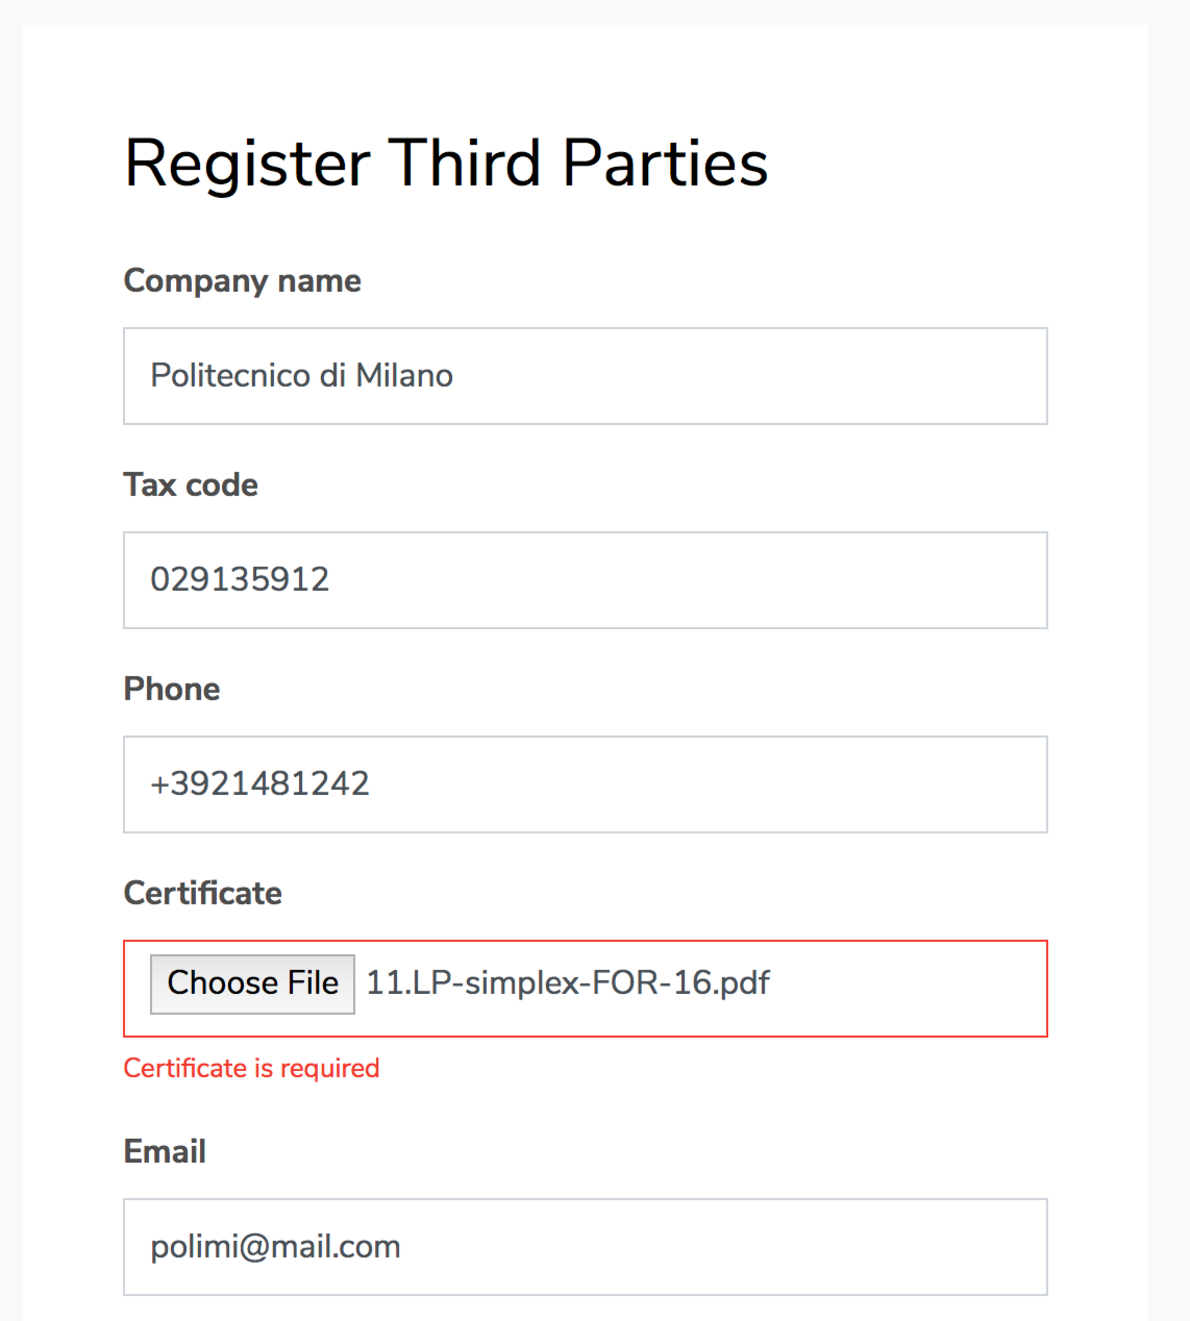
\includegraphics[width=0.6\linewidth]{images/certificateBug}
\centering
\caption{ UI Certificate bug }
\label{fig:certificatebug}
\end{figure}

\item 
The site is not responsive and can't be accessed, for instance, from a smartphone or from device with a resolution that is too low

\end{itemize}